\documentclass[border = 0.2cm]{standalone}

% Required packages and libraries
\usepackage{tikz}
\usetikzlibrary{positioning,petri}

\begin{document}

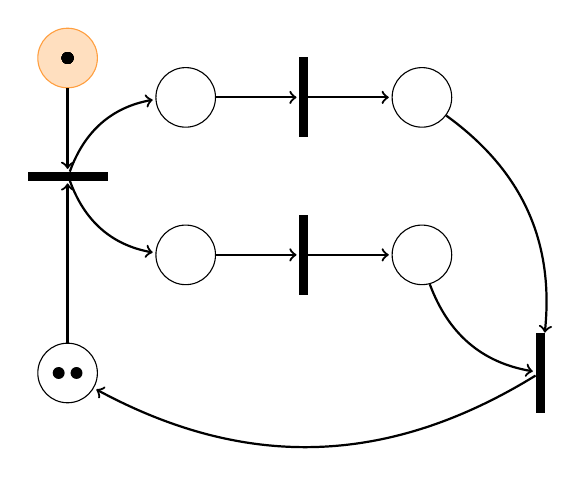
\begin{tikzpicture}[node distance=3cm,on grid]

% Input data
\node[place,
	fill=orange!25,
	draw=orange!75,
	tokens=10] (cond_to_be_processed) {};
	

\node[transition,
	below= 1.5cm of cond_to_be_processed,
	minimum height=1mm,
	minimum width=10mm,
	fill=black] (read) {};

%%%%%%%%%%%%%%%%%%%
% Post-read buffers

\node[place, above right= 1cm and 1.5cm of read] (cond_cipher) {};
\node[place, below right= 1cm and 1.5cm of read] (cond_rcount) {};

\node[transition,
	right= 1.5cm of cond_cipher,
	minimum height=10mm,
	minimum width=1mm,
	fill=black
] (cipher) {};
	
\node[transition,
	right= 1.5cm of cond_rcount,
	minimum height=10mm,
	minimum width=1mm,
	fill=black
] (rcount) {};


\draw[thick] 
    (read) edge[post, bend left=30] (cond_cipher)
    (read) edge[post, bend right=30] (cond_rcount)
    (cond_cipher) edge[post] (cipher)
    (cond_rcount) edge[post] (rcount);

%%%%%%%%%%%%%%%%%%%
% Read processed buffers

\node[place, right= 1.5cm of cipher] (pcond_cipher) {};
\node[place, right= 1.5cm of rcount] (pcond_rcount) {};
	
\draw[thick] 
    (pcond_cipher) edge[pre] (cipher)
    (pcond_rcount) edge[pre] (rcount);
	
%%%%%%%%%%%%%%%%%%%
% Read resources

\node[place,
	below=2.5cm of read,
	tokens=2] (cond_readbuf) {};
	
\draw[thick]
    (cond_readbuf) edge[post] (read)
	(read) edge[pre] (cond_to_be_processed);

\node[transition,
	below right= 1.5cm and 1.5cm of pcond_rcount,
	minimum height=10mm,
	minimum width=1mm,
	fill=black
] (reclaim_readbuf) {};

	
\draw[thick] 
    (pcond_cipher) edge[post, bend left=30] (reclaim_readbuf)
    (pcond_rcount) edge[post, bend right=30] (reclaim_readbuf)
    (reclaim_readbuf) edge[post, bend left=30] (cond_readbuf);



% Transition 1
% \node[transition,
% 	below left= 1.5cm and 1cm of place1,
% 	minimum height=1mm,
% 	minimum width=10mm,
% 	fill=black,
% 	label=left:$T_1$] (trans1) {};

% Transition 2
% \node[transition,
% 	below right= 1.5cm and 1cm of place1,
% 	minimum height=1mm,
% 	minimum width=10mm,
% 	fill=black,
% 	label=right:$T_2$] (trans2) {};

% Connect P1-T1-P2-T2-P1
% \draw[thick] (place1) edge[post,bend right=30] (trans1)
% 	(trans1) edge[post,bend right=30] (place2)
% 	(place2) edge[post,bend right=30] (trans2)
% 	(trans2) edge[post,bend right=30] (place1);

\end{tikzpicture}

\end{document}
